% mn2esample.tex
%
% v2.1 released 22nd May 2002 (G. Hutton)

\documentclass[useAMS,usenatbib]{mn2e}
\usepackage{graphicx}
\usepackage{aas_macros}
\usepackage{multirow}
\usepackage{hyperref}
\usepackage{commath}
\usepackage{amsmath}
\usepackage{subfig}
\usepackage{pdflscape}
%\usepackage{epstopdf}


%%%%% AUTHORS - PLACE YOUR OWN MACROS HERE %%%%%
\newcommand\ion[2]{\text{#1\,\textsc{\lowercase{#2}}}}

%%%%%%%%%%%%%%%%%%%%%%%%%%%%%%%%%%%%%%%%%%%%%%%%

\title[Deconstructing M83]{Deconstructing a galaxy: identifying components of M83 with photometric clustering%
\footnote{  
Based on observations made with the NASA/ESA Hubble Space Telescope, obtained from the Data Archive at the Space Telescope Science Institute, which is operated by the Association of Universities for Research in Astronomy, Inc., under NASA contract NAS 5-26555. These observations are associated with program \#11360.
}
}
\author[Kiar \& Barmby]
{
A. K. Kiar$^{1}$\thanks{E-mail: akiar@uwo.ca} and
P. Barmby$^{1}$\thanks{E-mail: pbarmby@uwo.ca}\\
$^{1}$Department of Physics and Astronomy and Centre for Planetary Science and Exploration,\\
University of Western Ontario, London, ON, N6A 3K7, Canada\\
}

\begin{document}

\date{}

%\pagerange{\pageref{firstpage}--\pageref{lastpage}} \pubyear{2002}

\maketitle
\label{firstpage}

\begin{abstract}
% Abstract
Space-based astronomical observatories generate vast quantities of data.
As technology advances, the size of surveys will grow, and efficient means of analyzing the data they produce are necessary.
Machine learning methods present an effective way to handle large datasets, and are becoming a popular way to analyze large surveys in astronomy.
The purpose of this research is to apply machine-learning methods to the classification of point sources in the nearby galaxy Messier 83 (M83).
The Early Release Science Program survey took observations over ten filters in the UVIS channel, from the Wide Field Camera 3 on the Hubble Space Telescope, in the range of Optical to Near Infrared.
Mean-shift, Affinity Propagation, and K-means, clustering methods were applied to observations of point sources in the M83 galaxy.
Colour-colour combinations were created and clustered.
Clustering was performed in two and three dimensions to determine the effectivness of clustering a typical survey.
To identify which colour combination was most effective at separating different classes of objects, the strength of the clustering was evaluated and the results compared with independent classification, to determine if objects were correctly identified.
The most successful combinations are discussed, and a process outlined for the application of these methods to future surveys.
The results of this work will allow astronomers to plan observations that can be used to automatically classify objects in nearby galaxies, leading to more effective surveying, and effecient use of data.
\end{abstract}

\begin{keywords}
  galaxies: individual: M83
  galaxies: photometry
  galaxies: stellar content
  methods: statistical
  catalogues % or surveys?
\end{keywords}

\section{Introduction}

\section{Introduction}


%\item Galaxies have a lot of discrete sub-components: stars, clusters, nebulae, nucleus.
Galaxies are complex systems, comprised of numerous components with an enourmous range of size,
mass, density, and composition.
These components can be divided into baryonic (stars and their remnants,
nebulae, star clusters, nucleus) and non-baryonic (dark matter);
cataloging the components and describing
the interactions between them is a key step in elucidating the natural history of galaxies.
Only in nearby galaxies can individual sub-components be resolved.
As observational technology has advanced,
the definition of ``nearby'' has changed and will continue to do so, from Milky Way satellites and Local Group galaxies, to a few
Megaparsecs \citep[distance at which stars can be resolved with HST][]{},
to XX Mpc \citep[distance at which stars can be resolved with JWST][]{},
to the entire observable universe with potential future facilities \citep{}.

%\item One way to isolate specific components is with narrow-band filters or CMD analysis.
What is the most efficient way to survey the sub-components of a nearby galaxy?
Here we are discussing components detectable in imaging at ultraviolet through infrared wavelengths,
i.e. with effective temperatures in the range XX--XX~K.
Much cooler or hotter types of objects (molecular gas, accreting compact objects) are better-detected at other wavelengths.
Particular stellar types, or star clusters, are often identified with broad-band colour-magnitude diagrams \citep[e.g.][]{}.
Narrow-band filters can also isolate special stellar types \citep[e.g.][]{} or objects prominent in emission
lines such as planetary nebulae or supernova remnants \citep[e.g.][]{}.
Observations are typically designed with detection of particular classes in mind and sometimes re-used for additional purposes \citep[e.g.][]{}.
Spectroscopic follow-up is often required to confirm candidates.
New observational facilities which provide spatially-resolved spectroscopy  \citep[e.g.]{}{} may reduce the need for separate imaging and follow-up steps,
but greatly increase the complexity of initial data analysis.


Multi-wavelength surveys are extremely common in studies of unresolved galaxies in the distant universe.
While these are often designed to select galaxies or active galactic nuclei with specific properties \citep[e.g.][]{},
sometimes they are pure blank-field surveys.
Broadband ($R=\Delta \lambda/\lambda \lesssim X$) filters are the most common imaging modality,
although there have been a few attempts at narrow- or medium-band surveys as well \citep[e.g.][]{combo-17},
Clustering in colour space can be used to select particular classes of objects from a survey,
for example in selecting AGN via mid-infrared colours \citep[e.g.][]{},
or high-redshift galaxies via Lyman-break dropouts \citep[e.g.][]{}. 
{\bf give some examples here of sophisticated analysis of colour spaces.}

%\item But what if you already have all the filters, and you want to make a census? 
%Can start with properties of known classes of objects \& pick out from multi-dimensional dataset.
%\item Another approach is to see what blind clustering gets you: how many groups and what are they?
%How does this depend on the (number of) wavelengths used?
The purpose of this work is to treat a nearby galaxy as if it were a blank field for surveys, and investigate the
usefulness of different photometric colours for identifying sub-components.
We make use of the Early Release Science (ERS) observations with the Wide-Field Camera 3 (WFC3) of the nearby spiral galaxy M83 \citep{}
and in particular the catalog of point sources produced by \citet{}.
We form colours from the photometric measurements in the catalog and apply several clustering techniques to two-colour datasets.
In conjunction with published catalogs of galaxy components, we identify the optimum parameters for clustering such a photometric dataset,
and the best choices of filter.




%Outline of intro:
%
%\begin{enumerate}
%\item Galaxies have a lot of discrete sub-components: stars, clusters, nebulae, nucleus.
%\item One way to isolate specific components is with narrow-band filters or CMD analysis.
%\item But what if you already have all the filters, and you want to make a census? Can start
%with properties of known classes of objects \& pick out from multi-dimensional dataset.
%\item Another approach is to see what blind clustering gets you: how many groups and what are they?
%How does this depend on the (number of) wavelengths used?
%\end{enumerate}
%
%Work to be cited: 
%\begin{itemize}
%\item astro applications of k-means clustering 
%\item astro applications of other ML techniques
%\item general bkg on galaxy constituents
%\item ??
%\end{itemize}

\section{Data}
\section{Data}

%\item intro to M83: global parameters (distance, size, environment)
The dataset used for this study is the Wide-Field Camera-3
Early Release Science (ERS) observations of the nearby spiral galaxy Messier 83 (M83).
M83 is a grand-design spiral of type SAB, located at a distance of 4.66~Mpc \citep{tully13}
and the largest member of the M83 subgroup of the nearby Centaurus group of galaxies \citep{tully15}.
The galaxy's apparent radius of $\sim12$~arcmin \citep{} is reasonably well-matched to the camera's field of view (XX true? XX)
{\bf And here we note some other interesting things about M83.}

%\item Intro to WFC3 ERS dataset
%\item existing studies with this dataset (cluster, massive stars, etc)
% ref: chandar10, section. TODO: check for (unintentional!) plagiarism
The objective of the ERS observations as a whole was to probe star formation in galaxies.
The observations of M83 were made in broad- and narrow-band filters in order to characterize both stellar and nebular properties.
They cover a $3.6\times3.6$~kpc$^2$ region in the northern portion of the galaxy, including the nucleus,
a portion of a spiral arm and an interarm region.
The spatial resolution of the images is $0\farcs0396$~arcsec~pixel$^{-1}$,
corresponding to a linear scale of $XX$~pc~pixel$^{-1}$ at the 4.66~Mpc distance.
A complete description of the observations and data processing is given by \citet{chandar10};
our work here uses the observations in the UVIS channel, listed in Table~\ref{tab:filters}.
A number of previous studies have used the ERS M83 dataset for various purposes.
These include studies of 
star clusters \citep{chandar10, wofford11, whitmore11, bastian11, bastian12, fouesneau12, silva13, andrews14, chandar14, adamo15,ryon15,hollyhead15, sun16},
H~{\sc ii} regions \citep{liu13}, supernova remnants and the interstellar medium \citep{dopita10, hong11, blair14, blair15}, 
resolved stars \citep{kim12, williams15},
and a super-Eddington off-nuclear black hole \citep{soria14}.


\begin{table}
\centering
\caption{
\label{tab:filters}}
\begin{tabular}{lll}
\hline\hline
Filter & Name & Exposure time\\
\hline
F225W &  Wide UV & 1800~s\\
F336W &  $U$-band & 1890~s\\ 
%F373N &  [\ion{O}{iii}] & 2400~s\\
F438W &  $B$-band & 1180~s\\
F487N &  H$\beta$ & 2700~s\\
%F502N &  [\ion{O}{ii}] & 2484~s
F555W &  V-band, South field & 1203~s\\
%F547M &  V-band, North field & \\
%F657N &  H$\alpha$+[\ion{N}{ii}]& 1484~s\\ 
%F673N &  [\ion{S}{ii}] & 1850~s\\
F814W &  $I$-band & 1203~s\\
\hline
\end{tabular}
\end{table}

We analyze the catalog produced by \citet{chandar10} and made available via **REF**.
The objects in this catalog were detected on a `white-light' image produced by a weighted combination of the $UBVI$ images.
Photometry in 0.5- and 3-pixel radius apertures at the positions of the detected sources was performed on the broad- and narrow-band images and tabulated in the Vega magnitude system. %TODO: pick one of the 2 apertures and just use that. AK: ideas on which one?
We apply the correction to the F657N magnitude zeropoint (from 20.72 to 22.35) noted in the header of the catalog.
\citet{chandar10} discussed aperture corrections for this catalog, but since we are primarily concerned with colours,
we omit any aperture corrections. %TODO: make sure this is a good idea.
The catalog contains about 68000 objects which are expected to include individual stars, star clusters,
supernova remnants, H${\sc ii}$ regions, planetary nebulae, %TODO: check that we expect these to be detectable!
stellar blends, and background galaxies. % TODO: anything else?
Completeness and reliability of the catalog are not discussed by \citet{chandar10},
but a visual inspection of the the detected sources on the white-light image suggests that %TO BE COMPLETED..
XX objects are flagged in the catalog as being problematic %TODO: AK please compute this number using flag column
and we remove them from our analysis.

Table~\ref{tab:cat_numbers} and Figure~\ref{fig:mag_unc} characterize the catalog in terms of measurements in individual filters.
Not all objects are detected in all filters;
Table~\ref{tab:cat_numbers} gives the number of objects for which photometry is reported in a given filter,
the number for which reported magnitude uncertainty is $0.2$~mag or less,
and the aperture magnitude at which the median magnitude uncertainty is $0.2$~mag. 
%TODO: think about whether 0.2 is the right number.
% Catalog header says ``The  errors are probably reasonable but have not been "normalized" to truth (by comparing  subexposures), so not recomm ended for use except in a relative scale.'' Chandar paper does not discuss mag uncertainties.
Figure~\ref{fig:mag_unc} shows the distributions of magnitudes and uncertainties in the individual filters.

%AK: please calculate numbers here. For the last column scipy.stats.binned_statistic is a good way to do this.
\begin{table}
\centering
\caption{
\label{tab:cat_numbers}}
\begin{tabular}{lrrlr}
\hline\hline
Filter & $N_{\rm obj}$ & $N_{\rm good}$ & $m_{\rm good}$ & $N_{\rm X-555}$\\
\hline
F225W &  N & N & m & N\\
F336W &  N & N & m & N\\
F373N &  N & N & m & N\\
F438W &  N & N & m & N\\
F487N &  N & N & m & N\\
F502N &  N & N & m & N\\
F555W &  N & N & m & N\\
F657N &  N & N & m & N\\
F673N &  N & N & m & N\\
F814W &  N & N & m & N\\
\hline
\end{tabular}
\end{table}

%AK: here's where the plots go.
\begin{figure*}
\centering
%\includegraphics{fig1}
\caption{Distribution of magnitudes and uncertainties for objects in the \citet{chandar10} M83 ERS catalog.}
\label{fig:mag_unc}
\end{figure*}

% TODO: discuss (this might also go in a different section)
Our analysis in this paper is primarily concerned with colours, rather than luminosities.
Uncertainties in colours are computed as the quadrature sum of the relevant magnitudes.
Observations in 10 bands allow the generation of 45 different colours,
but not all of these colours are likely to be useful in characterizing components of the galaxy.
As the F555W band has the most individual detections, %TODO: AK: is this true?
we initially compute colours relative to this band.
The last column of Table~\ref{tab:cat_numbers} gives the number of objects for which a `good' colour (uncertainty $<0.2$~mag) is available.
%TODO: may use different number than 0.2.



%Outline for data section
%%\begin{enumerate}
%\item Intro to WFC3 ERS dataset
%\item intro to M83: global parameters (distance, size, environment)
%\item existing studies with this dataset (cluster, massive stars, etc)
%\item description of catalog (is there a ref for this??)
%\item anything about these data we don't like/didn't use?

%\end{enumerate}


\section{Methods}
%\section{Clustering Analysis}
As the size of galactic surveys grows, the number of dimensions available for analysis increases.
Clustering methods provide an efficient way of finding structure in high dimentional data by searching for structure in colour spaces that are difficult to visualize. 
The following techniques were used to cluster the data.
All analysis was implemented using the \textit{sklearn.cluster} Python package. \textbf{how do we cite this?} 

\subsection{Mean Shift Clustering} 
Mean Shift is a non-parametric clustering technique that is based on probability density function estimates at each point in the data. % Should we mentioned sklearn.cluster as the implementation? 
Mean Shift is a very powerful algorithm, but has not been widely used in astronomy. % Find a paper using it
Because Mean Shift moves towards the local mode near the data on which it was initialized, it is useful for estimating the number of signifcant clusters in a dataset \citet{comanciciu02}
At each point, the algorithm estimates the density around that point using a small sample of objects surrounding the point.
The power of Mean Shift clustering is that the clusters are not confined to a particular shape.
The algorithm is based on two components: kernal density estimation, and density gradient estimation.
We will highlight the major components of the algorithm, for a full description of the, see \citet{vatturi09}.

The first element of Mean Shift is kernel density estimation. 
The major parameter of Mean Shift is bandwidth, \textbf{\textit{H}}, which is assumed to be proportional to the matrix $\textbf{\textit{H}} = h^2\textbf{\textit{I}}$, with $h>0$ \citet{vatturi09}.
The desnity estimator for a multivariate density kernal is given by: 
\begin{equation} 
\label{eq:ms_de}
\hat{f}(x) = \frac{c_{k,d}}{nh^d} \sum_{i=1}^n k\Bigg( \norm{\frac{x-x_{i}}{h}}^2 \Bigg)
\end{equation}
Where $h$ is the magnitude of the bandwidth matrix, $k(x)$ is the profile of kernal $K(x)$, and $c_{k,d}$ is a constant making $K(x)$ integrate to one\citet{vatturi09}.
Estimating the bandwidth correctly is critical to determining the correct number of clusters.
If the bandwidth is too low, the density estimate will be undersmoothed, and Mean Shift will produce many small clusters \citet{vatturi09}. This is a result of the large density gradient resulting from a low bandwidth, causing many data points to be interpreted as local modes.
Conversly, if the bandwidth is too large, a small number of large clusters will be detected, resulting in groupings of data that may blur the underlying structure \citet{vatturi09}.

The second element of Mean Shift is density gradient estimation. 
The density gradient is estimated from the gradient of equation~\ref{eq:ms_de}\citet{vatturi09}.
The density gradient is given by: 
\begin{multline}
\label{eq:ms_dg}
\nabla\hat{f}_{h,K}(x) = \frac{2c_{k,d}}{nh^(d+2)} \Bigg[ \sum_{i=1}^n k^{\prime} \Bigg( \norm{\frac{x-x_{i}}{h}}^2 \Bigg) \Bigg] \\ \Bigg[\frac{\sum_{i=1}^n x_{i}k^{\prime} \Bigg( \norm{\frac{x-x_{i}}{h}}^2 \Bigg)}{\sum_{i=1}^n k^{\prime} \Bigg( \norm{\frac{x-x_{i}}{h}}^2 \Bigg)} - x \Bigg]
\end{multline}
The second term of equation~\ref{eq:ms_dg}, is the Mean Shift; the difference between the weighted mean using $k^{\prime}$, and $x$ \citet{vatturi09}.
Applying a normal kernal to the Mean Shift, the second term of equation~\ref{eq:ms_dg} becomes: 
\begin{equation} 
\label{eq:ms_sh}
m_{h,K}(x) = \frac{\sum_{i=1}^n x_{i} exp \Bigg(\norm{\frac{x-x_{i}}{h}}^2 \Bigg)}{\sum_{i=1}^n exp \Bigg(\norm{\frac{x-x_{i}}{h}}^2 \Bigg)} - x
\end{equation}
$m_{h,K}$ is the Mean Shift, and always points in the direction of largest ascent through the estimated density function \citet{vatturi09}.

Mean Shift clustering involves the application of equation~\ref{eq:ms_sh} to shift the points of a data set towards the direction of the Mean Shift vector \citet{vatturi09}. 
The points are shifted by: 
\begin{equation}
\label{eq:ms}
x^{i+1} = x^i + m_{h,K}(x^i)
\end{equation}
Shifting the data points by equation~\ref{eq:ms} ensures that when the points converge, the center is the area of highest local density, or density ``mode". 
The density mode can be interpretted as the center of a significant cluster in the data set, and is used to classify the objects that were shifted towards it.
% Add section about bandwidth estimation
% Discuss drawbacks

\subsection{Affinity Propagation Clustering}

Affinity propagation (AP) is a relatively new clustering technique developed by \citet{frey07}.
Here, we will breifly describe the main compoments of AP, for a full description of the technique, see \citet{frey07}.
AP takes the similarities between the data points as input for clustering, and uses a series of "messages" between data points to determine the number of clusters and their centers.
The centers of AP clustering are actual data points, called exemplars, which make it useful for clustering as it does not create average centers for each cluster. 
The first input required for AP are the \textit{preferences} of each data point which describes the likelihood of a data point to be chosen as an exemplar \citet{frey07}.
The preferences are a measure of the similarity between a point \textit{i} and a candidate exemplar \textit{k} defined by: 
\begin{equation}
\label{eq:sim}
s(i,k) = -\norm{x_i - x_k}^2
\end{equation}
Similarity values influence the number of clusters AP identifies, as the larger similarity values are likely chosen as eemplars \citet{frey07}.
Preference values could be estimated using the median value of the similarities, the minimum value, or randomized to see the effects over various clusterings \citet{frey07}.

Once the preference value is determined, two messages are computed between all the data points.
The first message is the "responsibility" $r(i,k)$, which is sent from point \textit{i} to candidate exemplar \textit{k}:\citet{frey07}

\begin{equation}
\label{eq:resp}
r(i,k) \leftarrow s(i,k) - max_{k^\prime s.t,  k^\prime \neq k} \{ a(i,k^\prime) + s(i,k^\prime) \}
\end{equation}

Responsibility measures the evidence of how suitable point \textit{k} is to be an exemplar of point \textit{i} \citet{frey07}, after considering other potential exemplars for point \textit{i}.
The "availability", $a(i,k^\prime)$ in equation~\ref{eq:resp}, is sent from candidate exemplar \textit{k} to point \textit{i} to compute the evidence for how appropriate it would be for point \textit{i} to choose candidate \textit{k} as an exemplar, considering evidence from other points that believe candidate \textit{k} should be their exemplar \citet{frey07}: 

\begin{equation}
\label{eq:avail}
a(i,k) \leftarrow min\Big\{ 0, r(k,k) + \sum\limits_{i^\prime s.t, i^\prime \notin \{i,k\}} max\{0, r(i^\prime, k)\}\Big\}
\end{equation}

The availabilities of all points are initialized to zero, and the first iteration of responsibilities are set to the input preferences \citet{frey07}. 
Each iteration updates equation~\ref{eq:resp} and equation~\ref{eq:avail} to determine the optimal exemplars for the data.

As the process iterates, for point \textit{i}, the value of \textit{k} that maximizes $a(i,k) + r(i,k)$ identifies \textit{i} as an exemplar if $k=i$, or gives the exemplar of point \textit{i} \citet{frey07}.
In order to ensure that the message passing does not cause numerical oscilations, the messages are damped as they are updated.
The previous message value is multiplied by a damping-factor $\lambda$, and $1 - \lambda$ multiplied by the update value is added.
The damping-factor has a value between zero and one, with a default value of 0.5 \citet{frey07}.

\subsection{K-Means Clustering}
K-Means clustering is one of the most widely used clustering methods and has been used to identify a wide range of interstellar and intergalactic objects. % List papers that have done so
It is simple, robust, and easy to implement when analyzing high dimentional spaces, making it a powerful way to analyze galactic surveys. 
Generally, k-means begins by selecting $k$ data points at random and deems these points cluster centers.
Each object in the data set is then assigned to a cluster center by computing the least-squares distance to each center.
K-Means aims to minimize the sum of squares within each cluster given by:
\begin{equation}
\label{eq:km_sos}
J = \sum_{n=1}^N \sum_{k=1}^K min \big( \norm{x_n - \mu_k}^2 \big)
\end{equation}
Each point, $x$, is then assigned to the cluster center with the lowest distance in equation~\ref{eq:km_sos}\citet{tammour16}.
Once all data points have been assigned, the centers are re-calculated by taking the average of all the points in each cluster. 
This process continues until the centers do not change after two consecutive iterations \citet{sanchez-almeida13}. 

% Discuss drawbacks
% K-Means requires the number of clusters to be inputed by the user. 
% This posses a challenge for high dimentional data, as the number of clusters cannot be estimated by visual inspection. 

\section{Analysis}
% Analysis section
In this section we will outline the process used for each of the clustering methods.
An aim of this work was to help astronomers determine which filters were best at identifying different types of objects in a survey. 
Since the average survey is limited to four filters, different combinations of four filters were used to construct colours for clustering. 
Colours were constructed using the difference between two wavelengths. For a given combination of four filters, all possible colour combinations were used. % Change as needed
The feature space was constructed in two and three dimensions, to add a layer of analysis that isn't typically found in colour-colour space.

\subsection{Clustering Process}
Clustering was performed using all three methods for each colour combination. 
The methods were used independantly and in unison in order to determine the optimal clustering.
The following process allowed the investigation of the effect of all paramters on each clustering technique, leading to an optimal clustering. 
\begin{enumerate}
\item \textbf{Mean-Shift:} Mean-Shift clustering was performed first by estimating the bandwidth paramter with the $estimate_bandwidth$ function in $scikit_learn$.
Following the initial clustering, a "bandwidth hierarchy" was created by performing the clustering again with bandwidth values between $\pm$ intervals of $0.1$ from the estimated bandwidth.

\item \textbf{AP:} Affinity Propagation clustering was then performed by setting the preferences to 10\% of the number of objects in the data set, and setting the damping factor to $0.95$.
Following that clustering, an "Affinity hierarchy" was created by varrying the damping factor, and preference value to determine the effect of each parameter. 

\item \textbf{K-Means:} K-Means clustering was performed last.
The first two clusterings were performed using the number of clusters determined from the initial clusterings by Mean-Shift and AP.
Next, K-Means was performed with $K = \pm 4$ from the original clustering. 
\end{enumerate}
\subsection{Selecting the Clustering}
In order to determine the optimal clustering, a series of metrics were used.
For each clustering, the silhouette score, cluster centers, root mean square, average and standard devation of each colour, and the distances between points in each cluster were calculated. 
\subsubsection{Silhouette Score}
The silhouette score is a metric used to describe the compactness of a cluster in a given clustering and is calculated as an average of all samples in a clustering.  
The silhouette score is given by:
\begin{equation}
\label{eq:ss}
Silhouette Score = \frac{b - a}{\textit{max}\big(a, b\big)}
\end{equation}
where $a$ is the mean intra-cluster distance, and $b$ is the distance between a point and the nearest cluster that point is not a member of.
In addition to the average score of the clustering, the average score for each cluster within the clustering was computed.
The cluster score determines what is driving the average score, and uncovers which clusters are most compact.

\subsubsection{Cluster Statistics}
Various statistics were calculated for each cluster within a clustering to help describe the similarity between the objects in a given cluster.
The standard deviation and average colour was calculated for each colour and each cluster within a clustering. 
These metrics describe the distribution of the objects in the colour-colour space within a cluster. 
Clusters that had large standard deviations were viewed as too dissimilar to be a meaningful cluster, and the clustering parameters were changed or the clustering was removed. 
Clusters whose averages and medians were not close were also discredited. 

The fractional sizes of each cluster were also calculated.
This metric describes the distribution of objects between clusters, and provided a complete way to evaluate a given clustering. 
If a clustering segmented the objects into a large cluster followed by several smaller ones, the clustering was investigated further, as this segmentation could mean one of two things. 
This type of clustering could be a result of the identification of interesting objects, in which case the clustering algorithm was able to identify the objects and place them in the same cluster.
However, this type of clustering could also be a result of the underlying distribution of the data, as the clustering techniques are largely drawn to areas of high density.
If this is the case, the clustering only created the smaller clusters as a result of the parameters imposed on the clustering.

\subsubsection{Parameter Relationships}
Aside from metrics, the relationships between various metrics were investigated to determine the optimal clustering.
Figure~\ref{fig:sscore} shows the relationship between the silhouette score and the number of clusters imposed on the data for each type of clustering. 
The optimal number of clusters is found where the relation flattens.
For K-Means, this point is between 5-10 clusters.
The Mean-Shift scores do not follow a similar distribution as K-Means, as the accuracy of Mean-Shift is more directly related to the bandwidth parameter, seen in Figure~\ref{fig:bwscore}.
\begin{figure*}
\centering
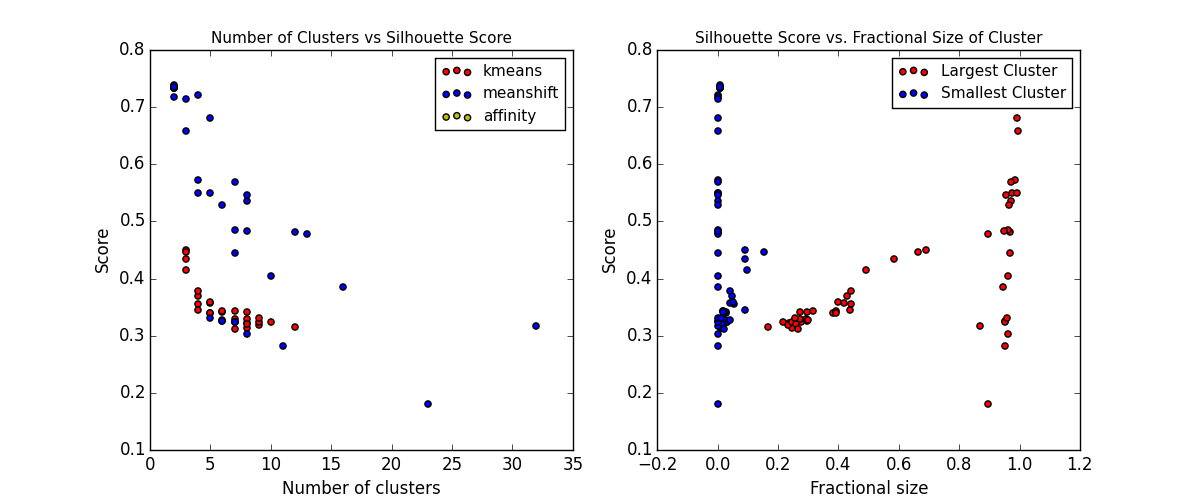
\includegraphics[width=0.5\textwidth]{figs/silhouette_score_relation}
\caption{Distribution of the silhouette score as a result of the number of clusters imposed. The \textit{blue} points are the scores of Mean-Shift clustering, \textit{red} points are scores of K-Means, and \textit{yellow} points are scores of AP.}
\label{fig:sscore}
\end{figure*}

\begin{figure*}
\centering
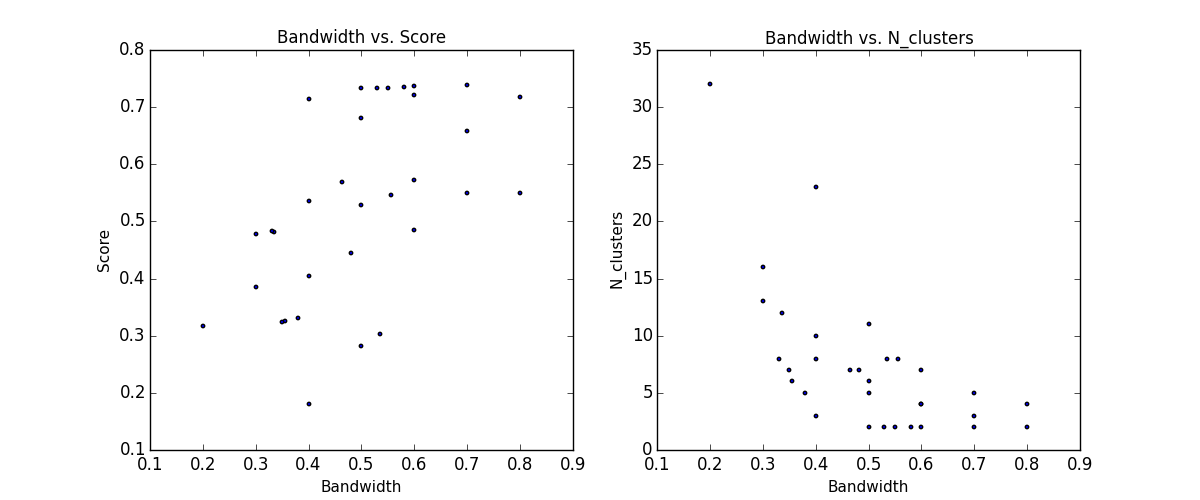
\includegraphics[width=0.5\textwidth]{figs/meanshift_parameters}
\caption{Distribution of the silhouette score as a function of bandwidth, and the distribution of the number of clusters as a function of bandwidth.}
\label{fig:bwscore}
\end{figure*}

\section{Results}
% Results section

\[ To be reorganized \]

The results of the analysis are grouped into the type of band used to make each colour.  % More general notes about results

\subsection{Broad \& Broad Band Combinations}
The four broad bands were used to create different colours. The only colour that was omitted from the analysis was the \textit{U - I} colour.
This was omitted because the range between those wavelengths is large enought that it is unlikely the ratio between the flux of those bands has any physical meaning.

\subsubsection{U - B vs. V - I}

\subsection{Broad \& Narrow Band Combinations}
Each broad and narrow band combination was tested against every broad-broad band combination that did not boarder the narrow band.

\subsubsection{UVW - U}
The UVW - U combination was tested clustered with the B-I, V-I, and B-V colours. % More general information about what we are looking for in this combination

\paragraph{Mean-Shift}
When clustered using Mean-Shift, a similar pattern of clustering was seen in all combinations.
Due to the structure of the Mean-Shift algorithm, it is drawn towards areas of high density in the distribution. % Refernce meanshift paper
Since the distribution of the UVW-U combinations were generally consentrated around zero in the colour-colour space, the Mean-Shift algorithm would pick out one large cluster with many smaller ones. 
Each smaller cluster had to be investigated to determine if the algorithm had found a meaningful cluster, or if it had just clustered noise.
In order to determine this, a cluster hierarchy was created with different bandwidth values to see how long each cluster lasted in the bandwidth space. 
If a small cluster was created at a low bandwidth level and stayed alive until the number of clusters became 2-3, then it is reasonable to assume that the cluster was meaningful.
Figure ~\ref{fig:UVWMS1} shows the result of one trial of Mean-Shift clustering with $h=0.6$ which created 4 clusters. 
Figure ~\ref{fig:UVWMS2} shows the result of one trial of Mean-Shift clustering with $h=0.4$, creating 10 clusters. 
The structure of cluster $2$ in both Figure ~\ref{fig:UVWMS1} and Figure ~\ref{fig:UVWMS2} can be seen distinctly. 
This cluster would have been viewed as noise if the hierarchy was not created, but after testing multiple bandwidth values, it can be seen that these objects are significant.
Varying the bandwidth did not have a large affect on the number of clusters produced. Bandwidth values from 0.5 to 1.0 only created a difference in three clusters generated. 

\begin{figure}
\centering
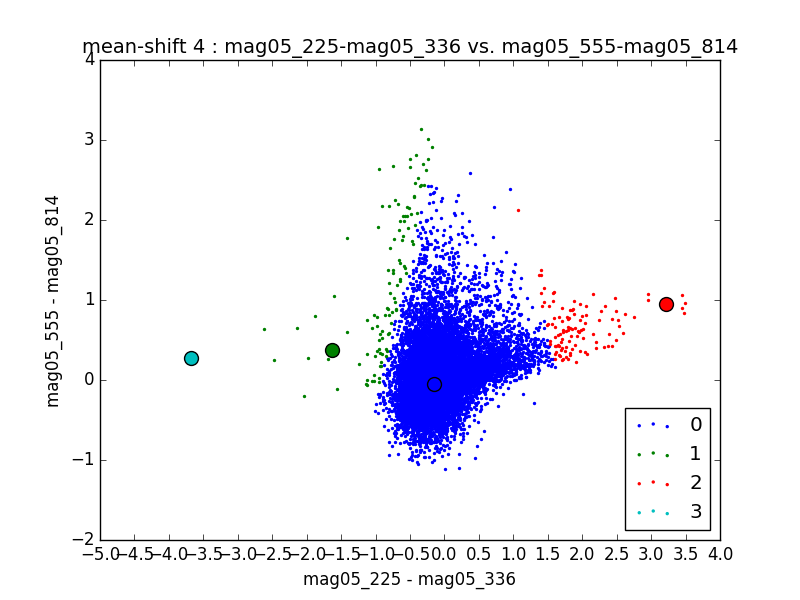
\includegraphics[width=\linewidth]{figs/meanshift_color_4cl_mag05_225-mag05_336vsmag05_555-mag05_814}
\caption{Colour-Colour distribution of the UVW-U and V-I colours, clustered using Mean-Shift with $h=0.6$. The colour of each point corresponds to the cluster the point was assigned to. Cluster numbers can be seen in the legend.}
\label{fig:UVWMS1}
\end{figure}

\begin{figure}
\centering
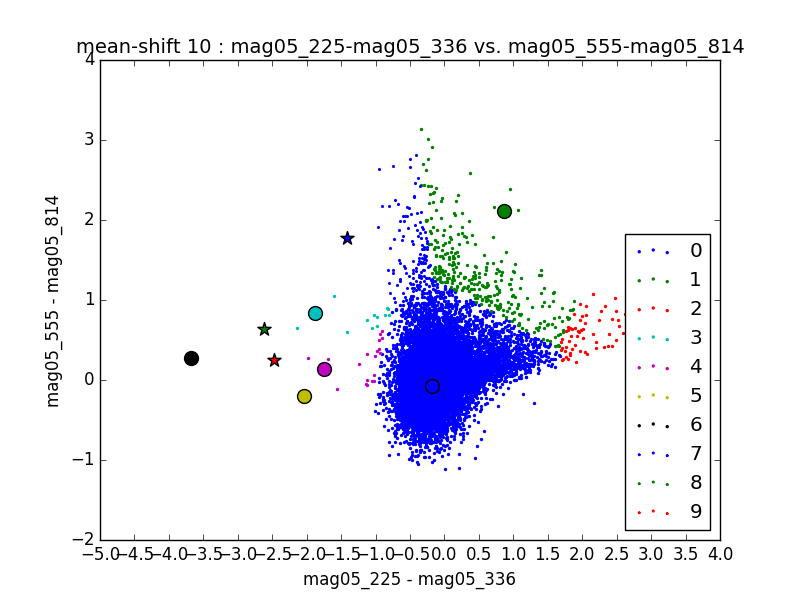
\includegraphics[width=\linewidth]{figs/meanshift_color_10cl_mag05_225-mag05_336vsmag05_555-mag05_814}
\caption{Colour-Colour distribution of the UVW-U and B-I colours, clustered using K-Means with $h=0.4$. The colour of each point corresponds to the cluster the point was assigned to. Cluster numbers can be seen in the legend.}
\label{fig:UVWMS2}
\end{figure}

\paragraph{K-Means}

When clustered using K-Means, two types of results were seen.
Figure ~\ref{fig:UVWKM1}, shows the result of K-Means clustering for $K=5$ against the B-V colour.

\begin{figure}
\centering
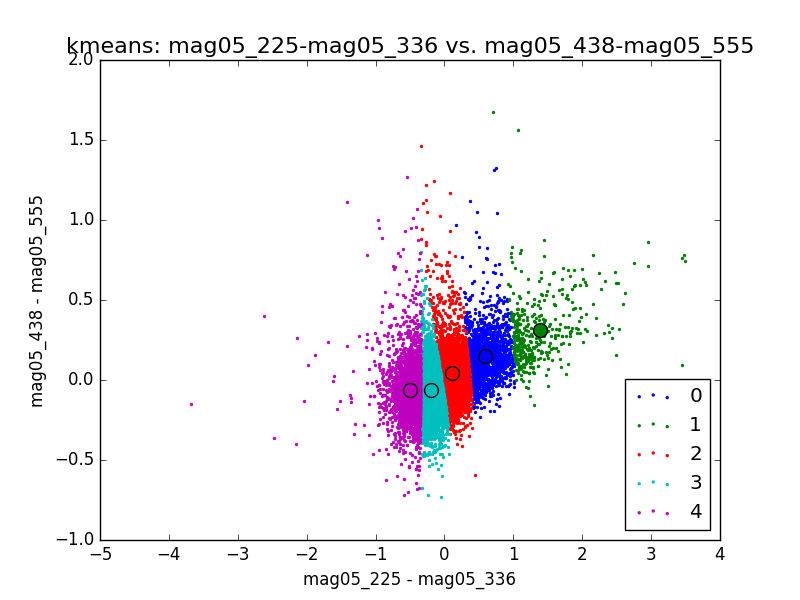
\includegraphics[width=\linewidth]{figs/kmeans_xy_5cl_mag05_225-mag05_336vsmag05_438-mag05_555}
\caption{Colour-Colour distribution of the UVW-U and B-V colours, clustered using K-Means with $K=5$. The colour of each point corresponds to the cluster the point was assigned to. Cluster numbers can be seen in the legend.}
\label{fig:UVWKM1}
\end{figure}

The algorithm split the data into groups based on its UVW - U colour. The pattern continued for all values of K, and the silhouette scores of the combination elbowed at $K=5$.
The second type of result for K-Means can be seen in Figure ~\ref{fig:UVWKM2}, against the B-I colour. 
This clustering segmented the data into circular groups within the distribution. 
Similar to the B-V combination, the silhouette score elbowed at $K=5$.

\begin{figure}[H]
\centering
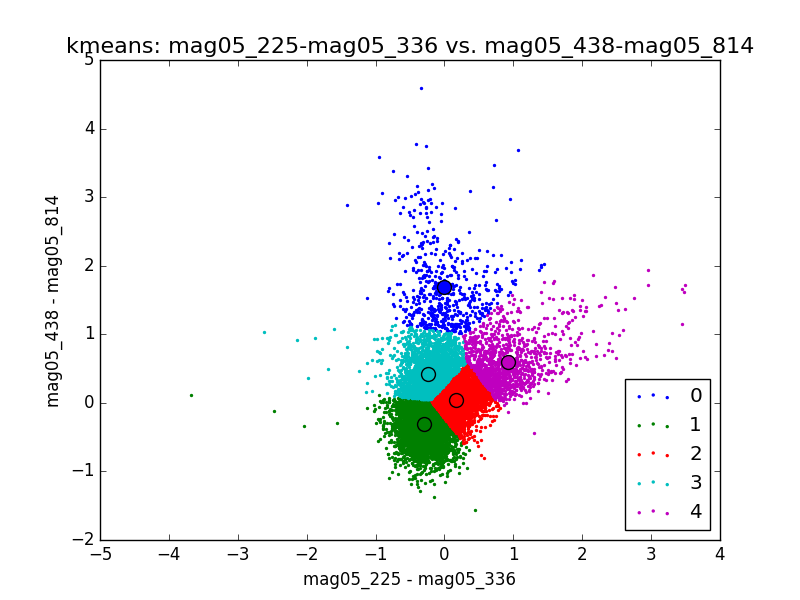
\includegraphics[width=\linewidth]{figs/kmeans_xy_5cl_mag05_225-mag05_336vsmag05_438-mag05_814}
\caption{Colour-Colour distribution of the UVW-U and B-I colours, clustered using K-Means with $K=5$. The colour of each point corresponds to the cluster the point was assigned to. Cluster numbers can be seen in the legend.}
\label{fig:UVWKM2}
\end{figure}

\paragraph{Astronomy Implications}
After the clustering was performed, the location of the cluster members were imposed on the whitelight image of M83.
The algorithms were able to identify sources that are located in unique sections of the galaxy.
K-Means segmented the data into objects that are located along the spiral arms exclusively, clustered in the denser regions of the arms and nucleus, and in the intra-arm region.
This pattern of object location was found through all combinations of broad - broad colours.
The Mean-Shift segmentation was able to identify objects that were located in the spiral arms.
The objects that were not part of the main cluster appear to be point sources that fall in the back of the galaxy, or are some form of cloud or dust.

\subsubsection{U - OII}
The U - OII combination was clustered with the B-V, B-I, and V-I colours using Meanshift followed by KMeans. % More general information about what we are looking for in this combination

\paragraph{2-Dimensions}

This colour seemed to be much more sensitive to bandwidth selection than other combinations.
With the B-V colour, $h=0.2$ produced $32$ clusters, while $h=0.4$ produced $3$. With the V-I colour, $h=0.35$ produced $17$ clusters, while $h=0.6$ produced $3$.
Due to this sensitivity, the bandwidth hierarchy was created on much narrower increases in $h$, which produced more meaningful clusters.
After producing the narrow hierarchy, the meanshift algorithm predictad a range of clusters from 3 to 13.
In each clustering, the algorithm did not seem to segment the data significantly, as similar to UVW - U, it produced one large cluster with several smaller ones.
The number of clusters predicted reduced linearly with the bandwidth selected, however, the silhouette score saw a sharp drop at $h = 0.33$, which produced 8 clusters, see Figure ~\ref{fig:UOIIMS}. 
This clustering segmented the data into three main groups, which were two "arms" in the distribution that spread to the redder areas of both colours.
Despite picking out these two groups, the two arms contained only approximately 5\% of the data and required further investigation. 

\begin{figure}
\centering
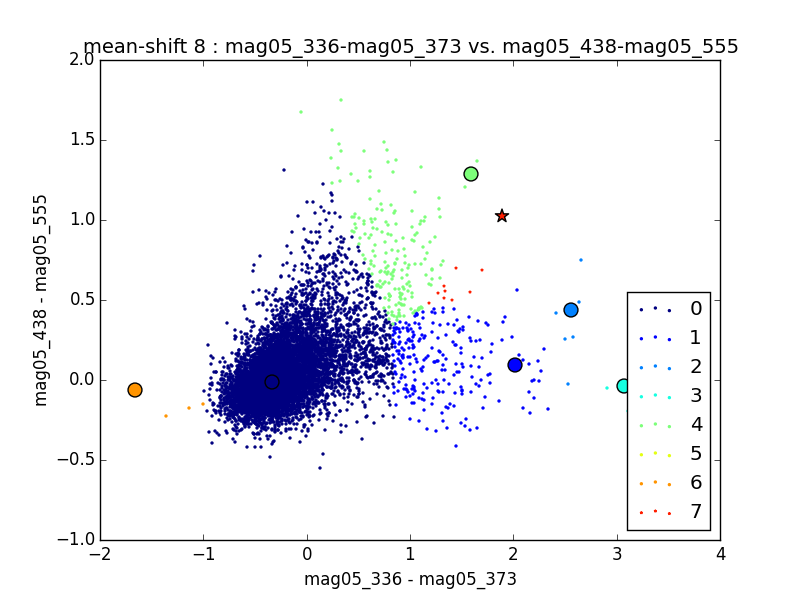
\includegraphics[width=\linewidth]{figs/meanshift_color_8cl_mag05_336-mag05_373vsmag05_438-mag05_555}
\caption{Colour-Colour distribution of the $U-O_{2}$ and B-V colours, clustered using Meanshift with $h=0.33$. The colour of each point corresponds to the cluster the point was assigned to. Cluster numbers can be seen in the legend.}
\label{fig:UOIIMS}
\end{figure}

The K-Means algorithm produced more reliable results, as it produced clusters of relatively similar sizes.
As K increased, the sum of squares value for each clustering decreased, a trend that is expected.
The silhouette score was a maximum at $K=3$, and elbowed at $K=5$. Both clusterings were investigated to determine which was optimal.
At $K=3$, the distribution was segmented according to its U - OII colour.
At $K=5$, the segmentation was similar, however, the section of data that was significantly red in the U-OII colour was given its own cluster.

With each combination of broad bands, the same patterns existed.
This combination in 2-Dimensions did not seem to uncover any more detail or interesting objects than the UVW-U combinations.

\paragraph{3-Dimensions}

Following the initial clustering, the colours were each broken down into a combination of the OII band and each other band.
The colours used in three dimensions were a combination of U-OII, OII-B, OII-V, and OII-I.

The clustering performance in three dimensions was generally better for almost all clustering parameters.
With all combinations, the clustering algorithms were able to identify a large branch of objects that was fairly red in the U-OII colour, and very blue in the other two, see Figure ~\ref{fig:UOIIKM3d}.
This branch was identified at all values of K, and most values of h.
The added complexity of three dimensions removed the restrictions of only using two dimensions, and allowed the algorithms to cluster the distributions more accurately.

\begin{figure}
\centering
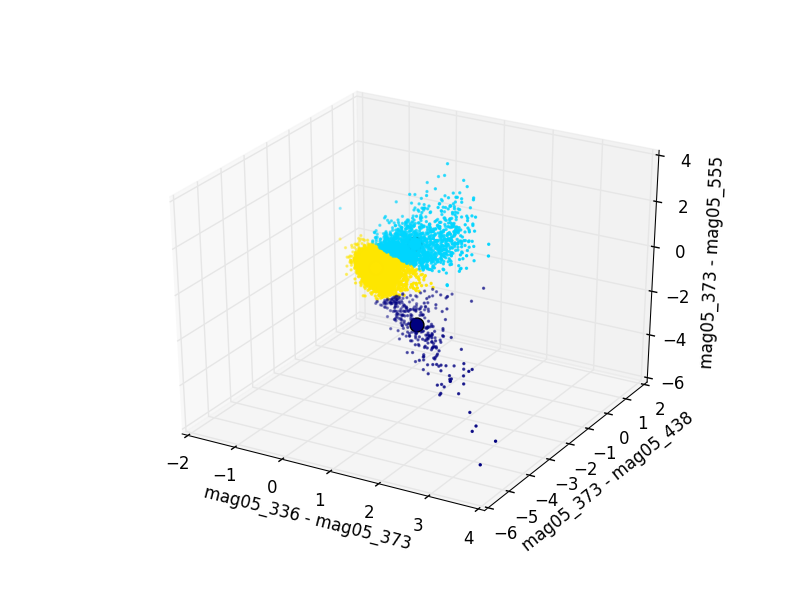
\includegraphics[width=\linewidth]{figs/kmeans_3d_color_3cl_mag05_336-mag05_373vsmag05_373-mag05_438vsmag05_373-mag05_555}
\caption{Colour-Colour distribution of the $U-O_{2}$, $O_{2}-B$, and $O_{2}-V$ colours, clustered using K-Means with $K=3$. The colour of each point corresponds to the cluster the point was assigned to. Cluster numbers can be seen in the legend.}
\label{fig:UOIIKM3d}
\end{figure}

The optimal meanshift clustering was not as apparent in three dimensions.
In the OII - B vs. OII - V combination, the score and number of clusters did not plateau, and the Meanshift clustering was not considered for the optimal clustering.
However, in the OII - B vs. OII - I and OII - V vs. OII - I combinations, the number of clusters elbowed at an h value that maximized the silhouette score.
The number of clusters elbowed at 5, over a range of h values for both combinations.
In each case, the algorithm was able to pick out groups of outliers more clearly than in two dimensions, and the elbow point was taken as the optimal meanshift clustering.

The K-Means algorithm was superior to meanshift for picking out evenly sized groups in all combinations, however, it was not able to pick out some of the detail lying in the groups of outlier data. 
In the combinations that meanshift was successful in, the score peaked at $K=4$, and this was chosen for the optimal clustering. In the last combination, the score peaked at $K=3$.
In addition, each K value was able to pick out the clear branch of objects.
When projected back into two dimensions, the successful segmentation of K-Means can be seen, as it identifies both branches of red objects, and the dense area around zero, see Figure ~\ref{fig:UOIIKM2d}.

\begin{figure}
\centering
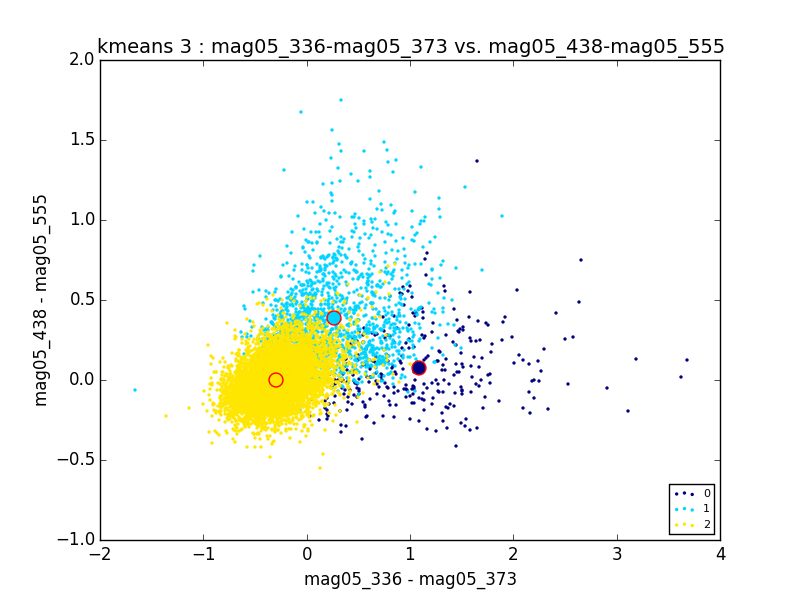
\includegraphics[width=\linewidth]{figs/kmeans_base_color_3cl_mag05_336-mag05_373vsmag05_438-mag05_555}
\caption{Colour-Colour distribution of the $U-O_{2}$ and B-V colours, projected from the 3D clustering using K-Means with $K=3$. The colour of each point corresponds to the cluster the point was assigned to. Cluster numbers can be seen in the legend.}
\label{fig:UOIIKM2d}
\end{figure}

\paragraph{Astronomy Implications}
Both 2 and 3 dimensional clusterings were investigated in the whitelight image. 
The clusterings in three dimensions were able to segment objects more diffinitively than two dimensions.
This was most noticable in the red branches of the distribution.
In two dimensions, the clusters that segmented the red branches seemed to be a combination of dim point sources and objects in the back of the galaxy or behind clouds.
In three dimensions, these clusters were almost entirely objects in the back of the galaxy or behind clouds instead of the combination.
Additionally, the clusters in three dimensions were better able to detect the boundary between the dense center of the distribution and the outlying branches.
When projected onto the galaxy, the objects dense center of the distribution were located in the densist areas of the spiral arms.
The three dimensional clusterings were able to identify these objects and keep them as a seperate cluster.

\subsubsection{B-H$\beta$}
The B-H$\beta$ colour was clustered with V-I in two dimensions, and H$\beta$-V, and H$\beta$-I in three dimensions.

\paragraph{2-Dimensions}
This combination was very sensitive to bandwidth selection. At $h=0.25$ the number of clusters predicted was 32, while at $h=0.4$, the number of clusters was four.
When selecting the optimal meanshift clustering, there was a significant drop in the number of clusters produced for the increase in bandwidth, which occured at $h=0.35$, giving eight clusters, see Figure ~\ref{fig:HBMS}.
This plateau was selected as the optimal clustering.
This selection did not maximize the silhouette score, but the trend in the score followed a similar pattern, and began to plateau at this level.

\begin{figure}
\centering
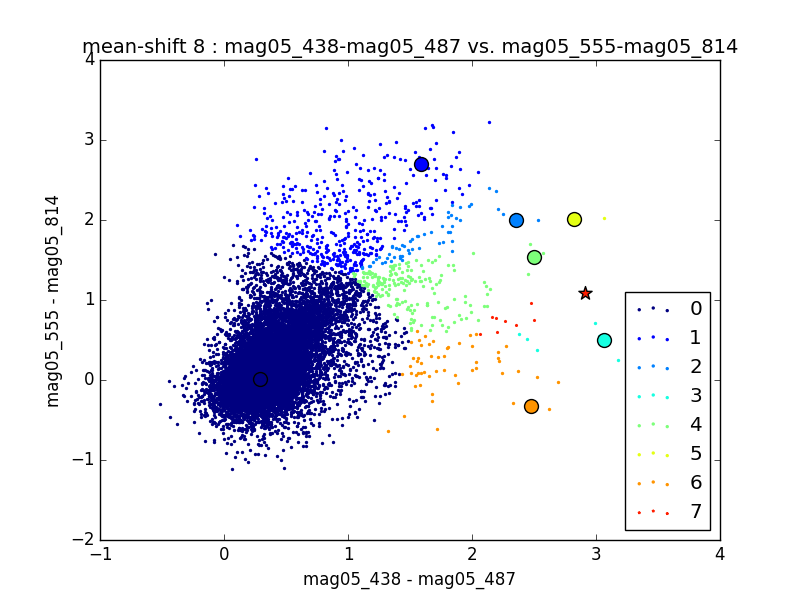
\includegraphics[width=\linewidth]{figs/meanshift_color_8cl_mag05_438-mag05_487vsmag05_555-mag05_814}
\caption{Colour-Colour distribution of the H$\beta$ and V-I colours, clustered using Meanshift with $h=0.35$. The colour of each point corresponds to the cluster the point was assigned to. Cluster numbers can be seen in the legend.}
\label{fig:HBMS}
\end{figure}

K-Means produced a segmentation that combined the results seen in previous trials.
The algorithm segmented the data in integers of the V-I colour, and was still able to create clusters for the redder branches of each colour.
The silhouette score plateaued at $K=5$ along with the sum of squares.
The algorithm was able to pick out the red branch in the B-H$\beta$ colour, however after further inspection, the score for that cluster specifically (which measures the cluster specific seperation from every other cluster) was quite low, indicating that the clustering was not as strong as the visual inpsection suggested.
This colour was the first combination to show clear structure in its corresponding colour-magnitude diagram (CMD).
Figure ~\ref{fig:HBCMD} shows the distribution of each cluster in the I vs. V-I space.

\begin{figure}
\centering
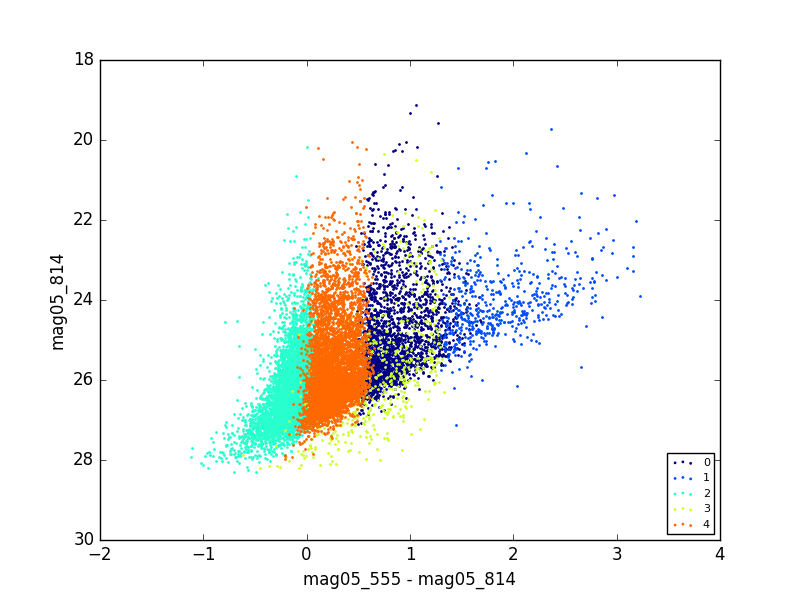
\includegraphics[width=\linewidth]{figs/kmeans_CMD_5cl_mag05_555-mag05_814vsmag05_814}
\caption{Colour-Magnitude distribution of the I and V-I bands, projected from a clustering using K-Means with $K=5$. The colour of each point corresponds to the cluster the point was assigned to. Cluster numbers can be seen in the legend.}
\label{fig:HBCMD}
\end{figure}

This CMD shows that this clustering was able to segmente the data based on its location in V-I colour space, and reveals detail about cluster 2, which has a magnitude cut-off at approximately 26.
Additionally, cluster 4, the red branch of B-H$\beta$, seems to sweep accross the magnitude distribution. % Need explaination of why

\paragraph{3-Dimensions}
The three dimensional clustering proved again to be more successful in segmenting the distribution. 
K-Means maximized the score at $K=4$, and was able to assign a clear branch of objects to its own cluster, see Figure ~\ref{fig:HBKM3d}.
Additionally, it was able to isolate the densist region of the distribution at zero, while identifying the group of objects very red in the V-I colour.

\begin{figure}
\centering
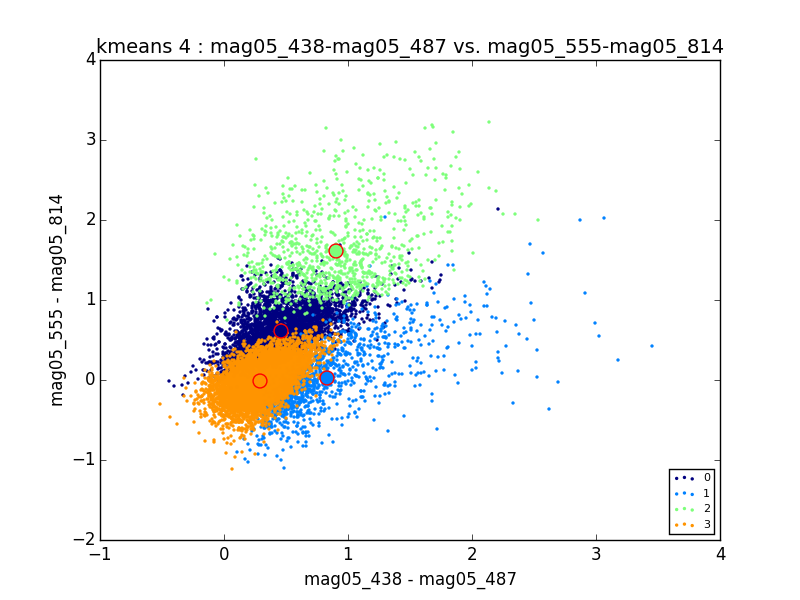
\includegraphics[width=\linewidth]{figs/kmeans_base_color_4cl_mag05_438-mag05_487vsmag05_555-mag05_814}
\caption{Colour-Colour distribution of the B-H$\beta$, and V-I colours, clustered using K-Means with $K=4$. The colour of each point corresponds to the cluster the point was assigned to. Cluster numbers can be seen in the legend.}
\label{fig:HBKM3d}
\end{figure}

Meanshift also performed well in three dimensions.
The relations between meanshift's parameters were not as clear as k-means, but the score plateaued at six clusters, which was chosen as the optimal clustering.
Meanshift was able to identify branches of objects that were clearly apparent in the three dimensional distribution, but also apparent as distinct segments of the H$\beta$-I, B-H$\beta$ distribution, see Figure ~\ref{fig:HB3dMS1} and Figure ~\ref{fig:HB3dMS2}.
Despite its ability to identify these groups, the main cluster detected by meanshift contained close to 96\% of the data.

\begin{figure}
\centering
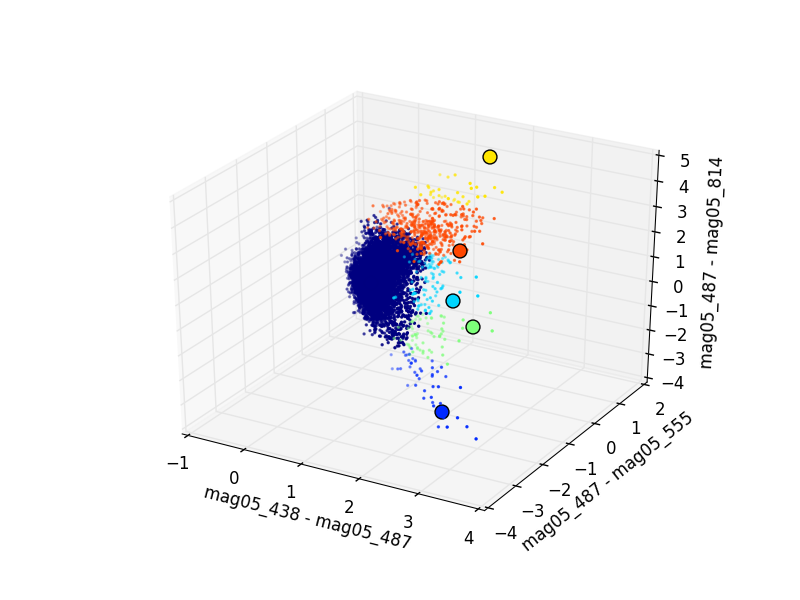
\includegraphics[width=\linewidth]{figs/meanshift_3d_color_6cl_mag05_438-mag05_487vsmag05_487-mag05_555vsmag05_487-mag05_814}
\caption{Colour-Colour-Colour distribution of the B-H$\beta$, H$\beta$-V, and H$\beta$-I colours, clustered using Meanshift with $h=0.65$. The colour of each point corresponds to the cluster the point was assigned to. Cluster numbers can be seen in the legend.}
\label{fig:HB3dMS1}
\end{figure}

\begin{figure}
\centering
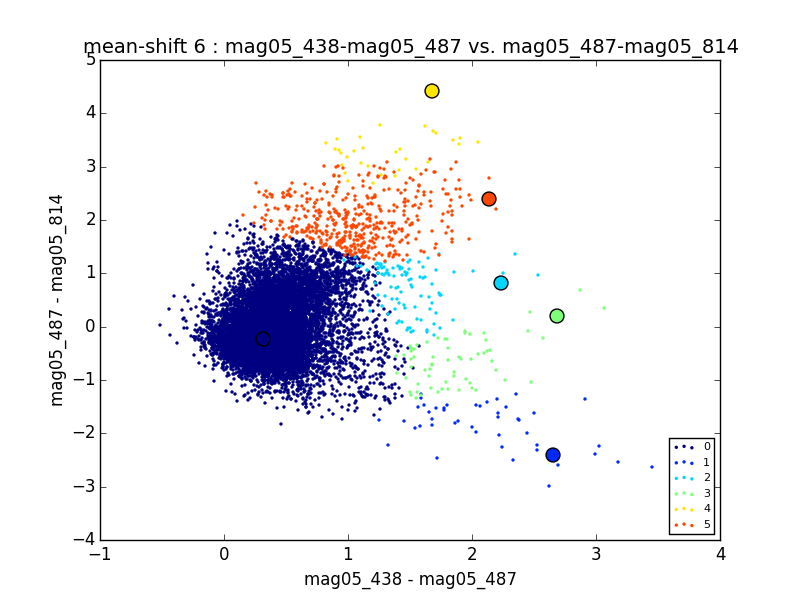
\includegraphics[width=\linewidth]{figs/meanshift_3d_color_6cl_mag05_438-mag05_487vsmag05_487-mag05_814}
\caption{Colour-Colour distribution of the B-H$\beta$ and H$\beta$-I colours, clustered using Meanshift with $h=0.65$. The colour of each point corresponds to the cluster the point was assigned to. Cluster numbers can be seen in the legend.}
\label{fig:HB3dMS2}
\end{figure}

\paragraph{Astronomy Implications}
While the two dimensional clustering seems to be more clearly defined in the colour-colour space, the three dimensional clustering seem to cluster objects that have similar colours, but also are very similar in their position in the galaxy.
Cluster two in Figure~\ref{fig:HBKM3d} is a group of dim point sources in some of the denser regions in the spiral arms. 
The similar cluster in two dimensions did not include regions of high density in the spiral arms, despite their similar colours.
The distribution of objects beyond the red arms remains similar to other colour combinations, where the main large cluster is associated with the densist areas of the spiral arms, and the second largest cluster is associated with the inter-arm region, and the nucleus.










\section{Discussion}
% Discussion

\textbf{This should be where we present a process for future surveys.}
\section{Conclusion}
% Conclusion

\textbf{Summarize paper}


\section*{Acknowledgments}

The authors acknowledge financial support from the Natural Science and Engineering Research Council (NSERC) of Canada.
This research has made use of the NASA/IPAC Extragalactic Database (NED) which is operated by the Jet Propulsion Laboratory,
California Institute of Technology, under contract with the National Aeronautics and Space Administration. 
This research has made use of the SIMBAD database, operated at CDS, Strasbourg, France.
We acknowledge the efforts of WFC3 Science Oversight Committee in conducting the Early Release Science program.

\appendix
\section{Published Catalogues}
%Appendix 1 - Published Catalgoues info

As one check on the results of our analysis, we use previously-published identifications of specific types of objects in M83.
We compiled a `published catalog' by combining the contents of the NASA Extragalactic Database (NED) and
[what does it stand for?] \citep[SIMBAD][]{wenger2000} and then adding the catalogs of Wolf-Rayet stars \citep{kim12} and
red supergiant candidates \citep{williams15}, which did not appear in either database.
NED's focus as an extragalactic database and SIMBAD's focus on Galactic objects mean that their contents overlap but are not identical, 
and this is true of the area surrounding M83. A $3\farcm3$ radius region around the coordinates centered at  ($204.26761\deg, -29.839939\deg$)
contains 1553 NED objects and 1772 SIMBAD objects, of which 1220 are matched with each other at 1\arcsec tolerance.
Although the two services use slightly different naming conventions, with human inspection the matches are generally recognizable as referring
to the same object. Interestingly, the databases do not always report the same object type even when the names are identical.
The differences are reasonable in some cases (a supernova remnant can also be an X--ray source, for example), but not others
(e.g. CXOU J133703.0-294945 is reported as a supernova remnant by SIMBAD and an H${\sc ii}$  region by NED).
A detailed study of the databases is beyond the scope of this work; for the purposes of this analysis, we kept the NED classification
for objects which appeared in both databases.
Objects which appeared in one database but not the other were primarily from recent work \citep[e.g.][]{long2014}, from
older studies likely superseded by newer ones \citep[e.g.][]{larsen1999}, or from studies in which only coordinates relative to
the galaxy centre were given \citep{rumstay83,dvpd83}.

Our final combined catalog has 2425 objects of which 750**check** are in the region covered by the ERS catalog.
The main classes are star clusters (350), X--ray sources (105), supernova remnants (86), H${\sc ii}$ regions (81),  and
radio sources (36).
Nearly every entry in the published catalog had an ERS catalog object within 1\arcsec, and the mean distance between
matched objects was 0\farcs26.
Given the nearly 100-fold difference in object density between the two catalogs, matching based on positions alone may 
result in spurious matches **REF**. *Some discussion of the exact matching procedure is warranted here, and a conclusion
on what the best thing to do is.**

\bibliographystyle{mn2e}
\bibliography{m83_refs}{}

\bsp

\label{lastpage}

\end{document}

